% This is the Reed College LaTeX thesis template. Most of the work
% for the document class was done by Sam Noble (SN), as well as this
% template. Later comments etc. by Ben Salzberg (BTS). Additional
% restructuring and APA support by Jess Youngberg (JY).
% Your comments and suggestions are more than welcome; please email
% them to cus@reed.edu
%
% See https://www.reed.edu/cis/help/LaTeX/index.html for help. There are a
% great bunch of help pages there, with notes on
% getting started, bibtex, etc. Go there and read it if you're not
% already familiar with LaTeX.
%
% Any line that starts with a percent symbol is a comment.
% They won't show up in the document, and are useful for notes
% to yourself and explaining commands.
% Commenting also removes a line from the document;
% very handy for troubleshooting problems. -BTS

% As far as I know, this follows the requirements laid out in
% the 2002-2003 Senior Handbook. Ask a librarian to check the
% document before binding. -SN

%%
%% Preamble
%%
% \documentclass{<something>} must begin each LaTeX document
\documentclass[12pt,twoside]{reedthesis}
% Packages are extensions to the basic LaTeX functions. Whatever you
% want to typeset, there is probably a package out there for it.
% Chemistry (chemtex), screenplays, you name it.
% Check out CTAN to see: https://www.ctan.org/
%%
\usepackage{graphicx,latexsym}
\usepackage{amsmath}
\usepackage{amssymb,amsthm}
\usepackage{longtable,booktabs,setspace}
\usepackage{chemarr} %% Useful for one reaction arrow, useless if you're not a chem major
\usepackage[hyphens]{url}
% Added by CII
\usepackage{hyperref}
\usepackage{lmodern}
\usepackage{float}
\floatplacement{figure}{H}
% Thanks, @Xyv
\usepackage{calc}
% End of CII addition
\usepackage{rotating}

% Next line commented out by CII
%%% \usepackage{natbib}
% Comment out the natbib line above and uncomment the following two lines to use the new
% biblatex-chicago style, for Chicago A. Also make some changes at the end where the
% bibliography is included.
%\usepackage{biblatex-chicago}
%\bibliography{thesis}


% Added by CII (Thanks, Hadley!)
% Use ref for internal links
\renewcommand{\hyperref}[2][???]{\autoref{#1}}
\def\chapterautorefname{Chapter}
\def\sectionautorefname{Section}
\def\subsectionautorefname{Subsection}
% End of CII addition

% Added by CII
\usepackage{caption}
\captionsetup{width=5in}
% End of CII addition

% \usepackage{times} % other fonts are available like times, bookman, charter, palatino

% Syntax highlighting #22
  \usepackage{color}
  \usepackage{fancyvrb}
  \newcommand{\VerbBar}{|}
  \newcommand{\VERB}{\Verb[commandchars=\\\{\}]}
  \DefineVerbatimEnvironment{Highlighting}{Verbatim}{commandchars=\\\{\}}
  % Add ',fontsize=\small' for more characters per line
  \usepackage{framed}
  \definecolor{shadecolor}{RGB}{248,248,248}
  \newenvironment{Shaded}{\begin{snugshade}}{\end{snugshade}}
  \newcommand{\AlertTok}[1]{\textcolor[rgb]{0.94,0.16,0.16}{#1}}
  \newcommand{\AnnotationTok}[1]{\textcolor[rgb]{0.56,0.35,0.01}{\textbf{\textit{#1}}}}
  \newcommand{\AttributeTok}[1]{\textcolor[rgb]{0.77,0.63,0.00}{#1}}
  \newcommand{\BaseNTok}[1]{\textcolor[rgb]{0.00,0.00,0.81}{#1}}
  \newcommand{\BuiltInTok}[1]{#1}
  \newcommand{\CharTok}[1]{\textcolor[rgb]{0.31,0.60,0.02}{#1}}
  \newcommand{\CommentTok}[1]{\textcolor[rgb]{0.56,0.35,0.01}{\textit{#1}}}
  \newcommand{\CommentVarTok}[1]{\textcolor[rgb]{0.56,0.35,0.01}{\textbf{\textit{#1}}}}
  \newcommand{\ConstantTok}[1]{\textcolor[rgb]{0.00,0.00,0.00}{#1}}
  \newcommand{\ControlFlowTok}[1]{\textcolor[rgb]{0.13,0.29,0.53}{\textbf{#1}}}
  \newcommand{\DataTypeTok}[1]{\textcolor[rgb]{0.13,0.29,0.53}{#1}}
  \newcommand{\DecValTok}[1]{\textcolor[rgb]{0.00,0.00,0.81}{#1}}
  \newcommand{\DocumentationTok}[1]{\textcolor[rgb]{0.56,0.35,0.01}{\textbf{\textit{#1}}}}
  \newcommand{\ErrorTok}[1]{\textcolor[rgb]{0.64,0.00,0.00}{\textbf{#1}}}
  \newcommand{\ExtensionTok}[1]{#1}
  \newcommand{\FloatTok}[1]{\textcolor[rgb]{0.00,0.00,0.81}{#1}}
  \newcommand{\FunctionTok}[1]{\textcolor[rgb]{0.00,0.00,0.00}{#1}}
  \newcommand{\ImportTok}[1]{#1}
  \newcommand{\InformationTok}[1]{\textcolor[rgb]{0.56,0.35,0.01}{\textbf{\textit{#1}}}}
  \newcommand{\KeywordTok}[1]{\textcolor[rgb]{0.13,0.29,0.53}{\textbf{#1}}}
  \newcommand{\NormalTok}[1]{#1}
  \newcommand{\OperatorTok}[1]{\textcolor[rgb]{0.81,0.36,0.00}{\textbf{#1}}}
  \newcommand{\OtherTok}[1]{\textcolor[rgb]{0.56,0.35,0.01}{#1}}
  \newcommand{\PreprocessorTok}[1]{\textcolor[rgb]{0.56,0.35,0.01}{\textit{#1}}}
  \newcommand{\RegionMarkerTok}[1]{#1}
  \newcommand{\SpecialCharTok}[1]{\textcolor[rgb]{0.00,0.00,0.00}{#1}}
  \newcommand{\SpecialStringTok}[1]{\textcolor[rgb]{0.31,0.60,0.02}{#1}}
  \newcommand{\StringTok}[1]{\textcolor[rgb]{0.31,0.60,0.02}{#1}}
  \newcommand{\VariableTok}[1]{\textcolor[rgb]{0.00,0.00,0.00}{#1}}
  \newcommand{\VerbatimStringTok}[1]{\textcolor[rgb]{0.31,0.60,0.02}{#1}}
  \newcommand{\WarningTok}[1]{\textcolor[rgb]{0.56,0.35,0.01}{\textbf{\textit{#1}}}}

% To pass between YAML and LaTeX the dollar signs are added by CII
\title{Radioresistant Bacteria of the Reed Research Reactor}
\author{Kaitlyn Li}
% The month and year that you submit your FINAL draft TO THE LIBRARY (May or December)
\date{May 2022}
\division{Mathematics and Natural Sciences}
\advisor{Jay Mellies}
\institution{Reed College}
\degree{Bachelor of Arts}
%If you have two advisors for some reason, you can use the following
% Uncommented out by CII
% End of CII addition

%%% Remember to use the correct department!
\department{Biochemistry and Molecular Biology}
% if you're writing a thesis in an interdisciplinary major,
% uncomment the line below and change the text as appropriate.
% check the Senior Handbook if unsure.
%\thedivisionof{The Established Interdisciplinary Committee for}
% if you want the approval page to say "Approved for the Committee",
% uncomment the next line
%\approvedforthe{Committee}

% Added by CII
%%% Copied from knitr
%% maxwidth is the original width if it's less than linewidth
%% otherwise use linewidth (to make sure the graphics do not exceed the margin)
\makeatletter
\def\maxwidth{ %
  \ifdim\Gin@nat@width>\linewidth
    \linewidth
  \else
    \Gin@nat@width
  \fi
}
\makeatother

% From {rticles}

\renewcommand{\contentsname}{Table of Contents}
% End of CII addition

\setlength{\parskip}{0pt}

% Added by CII

\providecommand{\tightlist}{%
  \setlength{\itemsep}{0pt}\setlength{\parskip}{0pt}}

\Acknowledgements{
I want to thank a few people.
}

\Dedication{
You can have a dedication here if you wish.
}

\Preface{
This is an example of a thesis setup to use the reed thesis document class
(for LaTeX) and the R bookdown package, in general.
}

\Abstract{
The preface pretty much says it all.

\par

Second paragraph of abstract starts here.
}

	\usepackage{setspace}\onehalfspacing
% End of CII addition
%%
%% End Preamble
%%
%
\begin{document}

% Everything below added by CII
  \maketitle

\frontmatter % this stuff will be roman-numbered
\pagestyle{empty} % this removes page numbers from the frontmatter
  \begin{acknowledgements}
    I want to thank a few people.
  \end{acknowledgements}
  \begin{preface}
    This is an example of a thesis setup to use the reed thesis document class
    (for LaTeX) and the R bookdown package, in general.
  \end{preface}
  \hypersetup{linkcolor=black}
  \setcounter{secnumdepth}{2}
  \setcounter{tocdepth}{2}
  \tableofcontents

  \listoftables

  \listoffigures
  \begin{abstract}
    The preface pretty much says it all.
    
    \par
    
    Second paragraph of abstract starts here.
  \end{abstract}
  \begin{dedication}
    You can have a dedication here if you wish.
  \end{dedication}
\mainmatter % here the regular arabic numbering starts
\pagestyle{fancyplain} % turns page numbering back on

\hypertarget{introduction}{%
\chapter*{Introduction}\label{introduction}}
\addcontentsline{toc}{chapter}{Introduction}

\hypertarget{significance}{%
\section{Significance}\label{significance}}

From medicine to insect control, fire alarms to renewable energy, nuclear technology has essential uses across a multitude of industries. In 1911, a young student named George de Hevesy lived modestly in Manchester while studying naturally radioactive materials. When dining with his landlady on a regular basis, he suspected that some meals were prepared with leftovers from many meals before. To test this hypothesis, he sprinkled a small amount of radioactive material into the leftovers, and the next day, found them in his meal using a rudimentary radiation detector. Hevesy went on to win the 1943 Nobel Prize and 1959 Atoms for Peace. This tracing application of radioactive materials is now widely used in industrial, medical, and environmental sciences. (1) But what about the health risks associated with radiation, one might ask?

Typically, when in close proximity to humans and health, nuclear technology tends to use substances with short half-lives. A half-life is the measurement of characteristic transformation over a period of time. For radioactive isotopes, this is a measurement of initial activity, where half of the initial is gone after the length of time specified as its half-life. (2) Radioactive iodine (I-123) has a half-life of 13 hours, so half of the original activity remains after 13 hours, then three-fourths after 26 hours, and seven-eights gone after 39 hours. This isotope of iodine is often a diagnostic tool for thyroid function, and the 13 hour half-life allows for it to decay quickly and no longer pose radiological dangers. (3) Longer living radioisotopes, such as most naturally occurring uranium (U-238) with a half-life of 4.5 billion years, are used in industries including low-carbon energy, water desalination, and food sterilization. (2)
As with all industries, hazardous waste needs a place to go and a method of safe disposal. Currently, there are many ways to deal with radioactive waste, such used fuel reprocessing and geological disposal facilities for safe decay. There have been many public doubts to these methods, citing transportation risks, long-term hazards, and emergence in future generations. In transport, radioactive waste is contained within tonnes of radiation- and corrosion-resistant material (such as stainless steel and lead), and typically vitrified so that the waste is immobile, insoluble, and stable for long periods of time. This allows for the materials to decay to the levels at which they were mined, and prevents leakage of contaminants into the environment. Short-term storage and disposal works well for wastes with multiple year half-lives. However, some wastes may need tens to thousands of year before decaying to naturally-occurring activity, which leads to issues of security and accessibility as time passes. (1)

Enter one of many solutions: the radioresistant microbe. Even in the most barren of places, bacteria can be found growing, maybe even thriving. If the world were explode and end, there would still probably be bacteria floating around just because they're so persistent. Thus, unsurprisingly, bacteria have been found in nuclear disaster sites such as Three Mile Island and Chernobyl. (4) Since initial considerations of radioresistant bacteria in industrial uses in 1996 (5), bacteria have been used to precipitate uranium contamination from groundwater (6) and reduce the oxidation state of uranium for metal leeching uses (7). Using radioresistant bacteria, decay and disposal of radioactive waste can be fast-tracked, and thousand-year storage can be avoided.

\hypertarget{radioresistant-spotlight}{%
\section{Radioresistant Spotlight}\label{radioresistant-spotlight}}

So what is radioresistance? Radioresistance refers the level of ionizing radiation an organism can withstand. High levels of radioresistance are often found among insects, worms, plants, and certain extremophiles such as \emph{Deinococcus radiodurans} (D. rad) and tardigrades. To give a reference point, a lethal dose of radiation to humans is between 4-10 Grays, whereas D. rad can withstand up to 15,000 Grays. Of course, there's a lot more complexities to the human body than to the single celled bacteria, but that is still many magnitudes more radiation in comparison. {[}noauthor\_radiochemistry\_nodate{]}

The biological effects of radiation have also been thoroughly studied since the atomic bombings in World War II. Scientists have found various different stochastic or deterministic effects, where a certain minimum dose of radiation is needed or the effect occur by chance, respectively. Radiation, ionization, and excitation can directly effect any part of the body, such as damaging specific protein molecules or nucleic acids. However, organisms mostly consist of water, so radiation directly mutating a single nucleic acid is rare. Instead, most radiation directly interacts with water, and the energy absorbed by the water creates highly reactive free radicals, which contain unpaired electrons (Figure \ref(fig:radiationDNA)). The unpaired electrons make free radicals highly reactive and chemically toxic to other molecules, in this case, other waters and free radicals. One possible chemical reaction is as follows:

The resulting hydrogen peroxide is a powerful oxidizing agent, and can thus affect molecules or cells that were not initially affected by radiation. While all organisms have some form of DNA or macromolecule repair mechanisms, most are not equipped for large scales of damage. Radiation damage is irreversible, so unless the damaged cells are quickly replaced by healthy ones, this can lead to the demise of organisms (2).

In 1956, the discovery of D. rad as a contaminant in radiation-sterilized corned beef cans brought about DNA-centered molecular biology (8). Radiosensitivity varies between quiescent and slow dividing cells versus cells with high proliferation rates. Like with growth-arrested bacteria and antibiotics, quiescent and slow dividing cells are less radiosensitive. Growth-arrested bacteria inactivate antibiotic targets, allowing the cells to remain dormant until the threat has passed. In slow growing cells, DNA repair mechanisms have the time to repair damage many times more than in standard growing species, allowing them to make sure every new cell is well-made. For example, D. rad is just as radiosensitive as many other bacteria, but due to its investment in efficiency of survival over growth, not only does it present spectacular DNA repair capacity for radioresistance, but also resistance to desiccation (8). Other organisms studied for radioresistance include \emph{Escherichia coli} (\emph{E. coli}), a less radioresistant bacteria found to produce resistant mutants based on environmental conditions and physiological factors, and melanin rich fungus found at the Chernobyl disaster site better protected against UV, solar, and ionizing radiation than its less pigmented relatives (9).

But as with any antibacterial method, extremophiles will form. Highly radioresistant strains of bacteria have been generated and found many times in environmental and laboratory settings. (11) In addition to that, there is also potential for microbial diversity induced by low levels of ionizing radiation to use as bioregenerative life support systems. (12) The study of these radioresistant bacteria and their robust cellular repair mechanisms are crucial for opening new doors in medicine, sustainability, and industry.

\hypertarget{the-reed-research-reactor}{%
\section{The Reed Research Reactor}\label{the-reed-research-reactor}}

Let's make this more local. Welcome to Reed College, we have a cute little tourist point call the Reed Research Reactor (RRR). It's a Training, Research, Isotopes, General Atomics (TRIGA) Mark I reactor built in 1968 by General Atomics primarily used for research and education. We're proudly the only nuclear reactor in the world that is owned and run by an exclusively undergraduate college. On the scale of reactors, it's small, underfunded, but well loved by the staff and community. Operators are officially licensed by the Nuclear Regulatory Commission (NRC), but since we're a non-profit educational institution, we're paid minimum wage.

Why do we have a reactor anyway? Reed does not have engineering as a major, much less nuclear engineering. Well you see, it all started with a murder. In 1934, Professor of Chemistry Ralph Kempton Strong left after accusations of murdering his wife arose, and Arthur F. Scott become a professor of chemistry at Reed in 1937. Scott's specialty was radiochemistry, and with the support from the Atomic Energy Commission (which has since been transformed into the NRC) eventually installed the reactor in 1968 {[}Ellis{]}. Since then, hundreds of students have been licensed, and hundreds of experiments have been conducted to their individual interests. Commonly mentioned experiments include irradiation of zebrafish, frog cells, fingernails, and archaeological artifacts to observe the effects of radiation on organism development and trace elements found in composite materials, respectively {[}gee\_effects\_2020{]}.

Let's do a quick crash course on radiation and health physics. Sometimes, atomic nuclei find themselves in unstable configurations due to energy imbalances or particle interactions. This instability makes the atom radioactive, so to relax and stabilize, the nucleus undergoes a process to lose energy by ejecting smaller particles or rearranging the protons and neutrons. The smaller particles containing energy are called radiation, and the process is radioactive decay. There are three types of ionizing radiation: alpha, beta, and gamma. Alpha particles are essentially a helium atom without electrons, composed of two protons and two neutrons. It's the heaviest of the three molecules, so it won't travel very far but will do a lot of damage if it gets to an unprotected area. This type of radiation is easiest to shield against---even the dead layer of cells covering your skin will do. Beta particles are similar to electrons, but ejected from the nucleus of an atom to turn a proton into a neutron, or absorbed to do the opposite. It's much lighter than the alpha particle, and can travel a little further, and need low atomic mass materials such as several inches of wood, plastic, or a sheet of aluminum foil to stop them. Lastly, gamma radiation is pure energy, completely mass-less. It can easily make its way through materials and needs a good amount of lead or concrete to shield it. Outside of ionizing radiation is neutron radiation. These particles don't ionize other atoms, instead the target can be made radioactive through a process called neutron activation to release one of three above ionizing radiations. Due to their neutral charge and lack of ionizing capabilities, neutrons are difficult to directly detect using typical hand-held radiation detectors such as Gieger-Mullers, and instead need various calculations or different instruments to accurately measure. To protect ourselves from them, we need three layers: one to slow it down (water), one to absorb it (boron), and one to shield from the resulting gammas released (concrete).

Why do we even want to shield ourselves from radiation? Atoms make up everything, so when the stability of an atom is disrupted, it can be like pulling the wrong piece out of a precariously balanced stack of blocks. In your body, the ionization radiation interacts mostly with water, which results in an unpaired election called free radical. This free radical is extremely reactive, so the slightly negatively charged water molecule will try to interact with anything it's close to, and since the body is 70\% water, there will be a lot of free radicals to mess with the status quo as mentioned previously. Tucked behind both a cell and nucleus membranes in eukaryotic cells is the vital molecule, deoxynucleic acid (DNA). DNA is the first component to the central dogma of biology, where it acts as the blueprint for the production of all other things---from proteins, to cells, tissue, organs, and organisms. Ionizing radiation and its results can destabilize membranes and the charged particles will interact with the DNA, causing base and sugar damage, single stranded breaks, and double stranded breaks. Double stranded breaks are often the most lethal, as chromosomal rearrangement can occur, repair is slow, and cell death or delayed mitosis can result. While there are many cell mechanisms that exist to repair these dangers, there can be too much damage and not enough time to effectively save the cell and its progeny.

Oh no, radiation sounds so scary! If I'm irradiated, can I turn into a non-trademarked superhero? Absolutely not. You might just die. Also, radiation is all around you! It's constantly emitted from sources such as the sun, the air, the ground, building materials, and even your food (13). A higher dose of radiation is receive on an airplane ride than the dose received while working at the reactor for the same amount of time. There is no escape.

\hypertarget{so-what-am-i-doing-here}{%
\section{So what am I doing here?}\label{so-what-am-i-doing-here}}

Well. The RRR core is situated in a 25000 gallon tank of filtered, demineralized water for optimal clarity and shielding for the various types of radiation. So with all the filtration and radiation, the reactor water should be pretty clean\ldots{} right?
Remember those extremophiles? Bacteria can survive off of just about anything, so even though there may not be explicit food for them in the water, there's plenty of materials that make up the reactor system itself. A study performed at the Three Mile Island nuclear power plant and the spent nuclear fuel pools of the Cofrentes nuclear power plant in Valencia, Spain, observed microbial growth living in ultra-pure, radioactive water. The nuclear industry started to devote attention to microbiological influenced corrosion of surfaces, but due to the belief that gamma radiation from the reactor fuel would effectively sterilize environments, the studies have been all but forgotten (14).

Inspired by Radioresistant microbes in the Reed Research Reactor (D. Dashevsky, Microbiology Lab Poster, Reed College, 2014), a short study by former microbiology student and reactor operator Daniel Dashevsky, we will isolate and identify bacteria from the primary filtration system of the Reed Research Reactor. In their project, Dashevsky isolated \emph{Pseudomonas fluorescens} ( \emph{P. fluorescens} ) from the reactor systems that demonstrated radioresistance. In Spring of 2021, samples were collected from various parts of the Reed Research Reactor (RRR) primary filtration system using sterile swabs and nutrient agar plates. Sampling areas included the primary filter and housing, the pool floor, the pool walls, poolside fuel racks, and the top of the core. While many strains of bacteria were isolated from the initial sampling of the RRR primary filtration system, only 5 strains from the primary filter (1°F1 - 5) were used for the irradiation in addition to the three controls: Dra, the radioresistant positive control; DDev, the RRR isolated radioresistant positive control; \emph{E. coli} strain DH5-\(\alpha\), the radiosensitive negative control. Overnight growths of these exposed to a dose of 877 µGy using a Cesium-137 source {[}insert activity{]} plated to observe differences in growth between irradiated and non-irradiated samples.

The result of this preliminary study reveal the potential of these bacteria and the RRR experimental systems to research radioresistant microorganisms. While the conclusions drawn from the study themselves do not reveal much, it allowed for experimental methods to be developed and refined for this thesis. In continuing the work, I have since found 3 strains of radioresistance \emph{Bacillus} species through UV irradiation and 16S analysis. Using the experimental facilities of the RRR, I hope to test and observe the hypothesis that the strains of radioresistant bacteria I find will contain robust DNA repair genes compared to standard lab strains to explain the basis of their radioresistance.

\hypertarget{mat-met}{%
\chapter{Materials and Methods}\label{mat-met}}

\hypertarget{initial-isolation}{%
\section{Initial Isolation}\label{initial-isolation}}

Samples were taken from the primary filter and surfaces of the Reed Research Reactor pool using sterile swabs and counting water on the way to the pool floor as part of sample collection. Swabs were attached to the end of a pole long enough to reach the bottom of the 25 feet deep pole, and after samples were collected, the cotton end of the swabs were broken off and put into tubes for transport to a sterile lab. Swabs were then used to grow lawns on nutrient broth agar plates (MilliporeSigma, St.~Louis, Mo) and isolated via streak purification. A total of 10 isolates were grown from the samples, but only strains 1\(^{\circ}\)F5, 1\(^{\circ}\)FH2, and CM1 were used for comprehensive growth and UV analysis.

\hypertarget{uv-testing-of-isolates}{%
\section{UV testing of isolates}\label{uv-testing-of-isolates}}

The bacterial strains and plasmids used in this study are listed in Table \ref{tab:isolates}. Liquid cultures were grown in lysogeny broth (LB: Tryptone 10 g/L, Sodium Chloride 10 g/L, Yeast Extract 5 g/L) at 37\(^{\circ}\)C and plated on LB agar plates for subsequent assays before another overnight growth.
\begin{longtable}[t]{lll}
\caption[Isolates of Focus]{\label{tab:isolates}Isolates of focus in this study}\\
\toprule
Strain & Genotype and Description & Source\\
\midrule
DH5-alpha & This is the negative control, a lab stock of \_Escherichia coli\_ used for recA1 mutation that makes this strain highly susceptible to radiation. Generously gifted by Dr. Jay Mellies. & Lab Strain\\
Deinococcus radiodurans (D. rad) & This is the positive control, a lab stock that is highly resistant to radiation. & Lab Strain\\
1°F5 & This is the fifth isolate from the primary filter of the Reed Research Reactor (RRR). & This study\\
1°FH2 & This is the second isolate from the primary filter housing of RRR. & This study\\
CM1 & This is the first isolate from the surface of the core and pool of RRR. & This study\\
\bottomrule
\end{longtable}
The initial UV testing of the original 10 isolates from Spring 2021 and two controls---D. rad and DH5-\(\alpha\)--- to compare the phenotype of these strains with D. Dev's initial results. Using an inoculating loop, overnight cultures were streaked across a plate superimposed on a grid for organization. Vertical quadrants of the plates were exposed for 0, 15, 30, or 60 seconds to 302 nm UV light using a 2 UV\(^{\text{TM}}\) Transilluminator (Analytik Jena GmbH, Jena, Germany) (see Figure \ref{fig:StreakUV}). Aluminum foil was used to shield unexposed or less-exposed areas, equally measured using the superimposed grid. After exposure, plates were incubated overnight at 30\(^{\circ}\)C and plate counts were performed.
\begin{figure}[t]
\centering
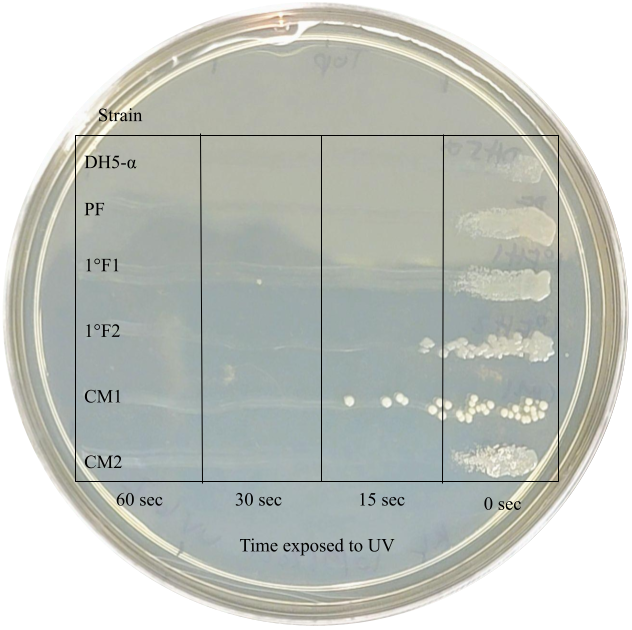
\includegraphics[width=\textwidth]{figure/StreakUV.png}
\caption[Streak UV]{Examples of how UV exposures were performed on plate streaks. For the 60 second streak, aluminum foil would cover up to the line between 60 and 30 seconds, and after 30 seconds, the aluminum foil would then move to cover the 15 and 0 second areas. After 15 seconds of exposing both the 60 and 30 second areas, the foil would again move to conceal only the 0 second area. After another 15 seconds, the exposure is complete so that each area receives the indicated time of exposure to UV. Note that several of these strains are not analyzed later in the study due to their lack of UV resistance.}
\label{fig:StreakUV}
\end{figure}
The secondary use of UV exposure was with serial dilutions of \(10^0\), \(10^{-1}\), \(10^{-2}\), \(10^{-3}\), \(10^{-4}\), \(10^{-5}\), and \(10^{-6}\) to observe percent survival of each 1\(^{\circ}\)F5, 1\(^{\circ}\)FH2, CM1, D. rad, and DH5-\(\alpha\). The dilutions were made using 1:10 ratios from \(10^0\) to \(10^{-5}\) in 1X Phosphate-Buffered Saline (PBS) (Sodium Chloride 8 g/L, Potassium Chloride 0.2 g/L, Sodium Phosphate Dibasic 1.44 g/L, Potassium Phosphate Monobasic 0.245 g/L, pH \(7.5 \pm 0.2\) at \(25^{\circ}\)C). In a sterile fume hood, 10 \(\mu\)L from each dilution was spotted onto plates superimposed on a grid and left to dry completely before inverting for UV exposure and incubation. Sets of three plates were exposed to UV for 0, 30, or 60 seconds gel-side-down, then incubated overnight at 30\(^{\circ}\)C. After incubation, colonies were counted and CFU/mL from serial dilutions was used to calculate percent survival across the different exposure times as shown with Equation \eqref{eq:psurvival}.
\begin{equation} 
  \text{Percent Survival} = \frac{\text{60 sec CFU/mL}}{\text{0 sec CFU/mL}} * 100% 
  \label{eq:psurvival}
\end{equation}
The third set of UV exposures was performed with normalized to \(2.2*10^5\) CFU/mL as the \(10^0\) dilution across all strains for better comparison of percent survival and growth rate of strains. This was to confirm that noted UV resistance was not just from quick growth rates or from high CFU/mL in the starting culture. Normalization was performed by growing overnights of each strain, plating serial dilutions, incubating overnight, then counting CFU/mL. The CFU/mL counted from the first plating was then used to dilute all fresh overnight liquid culture to approximately \(2.2*10^5\) CFU/mL for serial dilutions with UV exposure.

\hypertarget{s-pcr-analysis}{%
\section{16S PCR Analysis}\label{s-pcr-analysis}}

The following 16S primers in Table \ref{tab:primers} (15) were used to determine genus level classification of isolates. Prior to PCR, isolates were incubated overnight at 30\(^{\circ}\)C in nutrient broth.
\begin{verbatim}
Warning in read.table(file = file, header = header, sep = sep, quote
= quote, : incomplete final line found by readTableHeader on '/Users/
kaitlynli/Documents/Reed Year 4/Thesis/RRR_Bacteria/data/primers.csv'
\end{verbatim}
\begin{longtable}[t]{ll}
\caption[Primers]{\label{tab:primers}Primers used for 16S Analysis}\\
\toprule
Primer & Sequence(5'-3')\\
\midrule
SDBact0338aA18 & ACTCCTACGGGAGGCAGC\\
SDBact0515aA19 & GTGCCSGCMGCCGCGGTAA\\
SDBact1371aS20 & AGGCCCGGGAACGTATTCAC\\
SDBact1525aS17 & AAGGAGGTGATCCAGCC\\
\bottomrule
\end{longtable}
\begin{verbatim}
Warning in read.table(file = file, header = header, sep = sep, quote
= quote, : incomplete final line found by readTableHeader on '/Users/
kaitlynli/Documents/Reed Year 4/Thesis/RRR_Bacteria/data/pcr.csv'
\end{verbatim}
\begin{longtable}[t]{rll}
\caption[Primer Pairs]{\label{tab:pcr}Primers Pairs for PCR}\\
\toprule
Mix Number & Forward Primer & Reverse Primer\\
\midrule
1 & SDBact0338aA18 & SDBact1525aS17\\
2 & SDBact0515aA19 & SDBact1371aS20\\
3 & SDBact0515aA19 & SDBact1525aS17\\
\bottomrule
\end{longtable}
PCR was conducted to amplify 16S rRNA to assess microbial diversity using primers listed in Table \ref{tab:primers} and the combinations in Table \ref{tab:pcr} using Q5 High-Fidelity DNA Polymerase (New England BioLabs, Ipswich, MA) according to standard procedures. Cycling conditions (T100, Bio-Rad Laboratories, Hercules, CA) were 98\(^{\circ}\)C 40 sec, followed by varied cycles of 95\(^{\circ}\)C 10 sec, annealing temperature 55\(^{\circ}\)C 30 sec, 72\(^{\circ}\)C 30 sec.~Samples were run in duplicate for 30 cycles total.

DNA samples were separated on 25 mL 0.8\% agarose (Thermo Fisher Scientific Inc., Waltham, MA) in 1xTBE with 3 \(\mu\)L SybrSafe (Thermo Fisher Scientific Inc., Waltham, MA) at 90-120 V. 12 \(\mu\)L of PCR product was prepared with 3 \(\mu\)L volume 6X DNA gel loading mix (Thermo Fisher Scientific Inc., Waltham, MA) and run next to 250 ng of Quick-Load Purple 2-Log DNA ladder (0.1-10.0 kb) (New England BioLabs, Ipswich, MA). For controls, nuclease-free water was run in parallel to ensure the water used for primer master mixes was not contaminated.

The QIAquick Gel Extraction Kit (Qiagen Corp., Carlsbad, CA) was used to extract DNA from PCR products run on agarose gels to send in for sequencing of segments between 16S primer pairs. DNA fragments were excised as bands from agarose gel using scalpel on Transilluminator for visibility, and extraction was performed according to standard procedures. Product was sent to ACGT, Inc.~(Wheeling, IL) for sequencing, and resulting FASTA files were analyzed via SnapGene Viewer (GSL Biotech LLC, San Diego, CA) and run through NCBI nucleotide blasts for genus-level identification.

\hypertarget{growth-rate-analysis}{%
\section{Growth Rate Analysis}\label{growth-rate-analysis}}

To observe different growth rates independent of radioresistance, turbidity was measured by an Infinite 200 Pro microplate reader (Tecan, Männedorf, Switzerland) at 600 nm absorbance. Bacteria grown in LB were incubated at 30\(^{\circ}\)C for 24 hours at 30 minute intervals in a Greiner 96 Flat Bottom Transparent Polystyrene well plate (MilliporeSigma, St.~Louis, Mo). The doubling times were calculated from the slope of the most linear portions of the log of absorbance values. The equation is as follows:
\begin{equation} 
  \text{Doubling Time} = 0.301 * \frac{1}{\text{slope(sec)}} * \frac{60\text{sec}}{1 \text{min}} * \frac{60\text{min}}{1\text{hour}}
  \label{eq:doubling}
\end{equation}
\hypertarget{gram-staining}{%
\section{Gram Staining}\label{gram-staining}}

For inital characterization while awaiting 16S sequencing results from ACGT, Inc., samples were heat-fixed onto microscope slides by adding one drop of dH2O to slide and transferring a minute amount of a colony on solid media onto slide. For liquid cultures, one drop was transferred via inoculating loop. Mixture was spread evenly across 1.5 cm diameter circle and air dried. Using a clothespin, the slide was passed over a gentle flame to fix the cells. 5 drops of crystal violet stain were applied over the fixed culture and incubated for 60 seconds before rinsing with dH2O. Then, 5 drops of iodine solution were added, and incubated for 30 second before rinsing with dH2O. A couple drops of 95\% ethanol were used to decolorize the slide for no more than 5 seconds before rinsing with dH2O until solution ran clear. Slide was counterstained with 5 drops of safranin solution for 20 seconds and rinsed with dH2O before blotting dry to observed at 400x magnification (Olympus CH30, Olympus America Inc., Melville, NY). If the bacteria observed under a compound microscope were purple, they'd be Gram-positive. If the bacteria were pink or red, they'd be Gram-negative. All strains isolated and observed in this study were Gram-negative. The staining also aided in observing relative sizes.

\hypertarget{dna-sequencing-analysis}{%
\section{DNA Sequencing Analysis}\label{dna-sequencing-analysis}}

To prepare for while genome sequencing of strain CM1, the QIAGEN Genomic DNA (Qiagen Corp., Carlsbad, CA) handbook and kit were used according to procedure for bacterial samples. The isolated DNA was eluted in 1.5 mL nuclease free H\(_2\)O for sequencing and the concentration was determined using a NanoDrop ND-1000 spectrophotometer (Thermo Fisher Scientific Inc., Waltham, MA) to be around 14 \(\mu\)g/mL. A 500 \(\mu\)g/mL sample was sent to Novogene (Novogene Co, Davis, CA) for whole genome sequencing.

After a quality check using gel electrophoresis and a Qubit Fluorometer, raw data was read using an Illumina Sequence Identifier and cleaned up using a variety of internal quality control steps. The Burrows-Wheeler Aligner was utilized to map the paired-end clean reads to the reference genome of Priestia megaterium ASM993541v1 (16). Novogene then used the Genome Analysis Toolkit (Broad Institute, Cambridge, Massachusetts) to mark single nucleotide polymorphisms (SNP) and insertions or deletions from the mapped files, and then ANNOVAR (\url{https://annovar.openbioinformatics.org/en/latest/}) to annotate the different variants between the CM1 genome and the reference genome. Structural variants were isolated from the mapped genome files using breakdancer (\url{https://github.com/kenchen/breakdancer}) and ANNOVAR for annotation. Copy number variants were isolated using CNVnator (Bioinformaticshome.com) and ANNOVAR to annotate. A final report with results from above analysis was provided by Novogene, but the figures are not used in this study due to lack of niche understanding.

For whole genome sequencing, the isolated DNA is cut up into pieces and attached to specific adapters for the sequencing machinery. They're then read many times over and eventually, the genome is pieced together by observing overlapping sequencing that appear from the random fragmentation of the strands of DNA. After the genome is cleaned up and ready for analysis, programs compare it to the reference genome for differences such as single base pair changes (SNPs), places where parts of genes have been removed, replaced, or duplicated, and other general ways the analyzed genome is different from the reference.

After receiving the data from Novogene, the clean data files were uploaded to PATRIC Genome Assembly (\url{https://www.patricbrc.org/}) due to errors thrown when trying to annotate and map the information in a more user-friendly format than text files using RAST (\url{https://rast.nmpdr.org/}). RAST then was able to annotate and group the genes into subsystems for analysis and comparison of DNA metabolism mechanisms between the reference and CM1 genomes, as per the goal of this study. Using the SEED Viewer (\url{https://rast.nmpdr.org/seedviewer.cgi}) portion of RAST, the different genes for DNA metabolism and UvrABC system (DNA repair system in response to UV damage). The analysis performed on the genomic data was rudimentary due to time and experience restraints, but initial conclusions reveal endless paths for future studies.

\hypertarget{results}{%
\chapter{Results}\label{results}}

\hypertarget{radioresistance-part-1}{%
\section{Radioresistance? Part 1}\label{radioresistance-part-1}}

While many strains of bacteria were isolated from the initial sampling of the Reed Research Reactor (RRR) primary filtration system, only 3 strains from the Reed Research Reactor water system were used for the irradiation in addition controls \emph{Deinococcus radiodurans} (D. rad), the radioresistant positive control, and \emph{Escherichia coli} (\emph{E. coli}) strain DH5-\(\alpha\), the radiosensitive negative control. From UV-exposed serial dilutions of strains, CFU/mL were calculated and compared between strains using percent survival. With Figure \ref(fig:0secUV), the average CFU/mL calculated from colony counts across triplicate plates was used as the base, expected number of colonies if the strains were radioresistant. That number is then compared to the average CFU/mL for each strain in Figure \ref(fig:60secUV) as per Equation \ref{eq:psurvival}.
\begin{figure}[t]
\centering
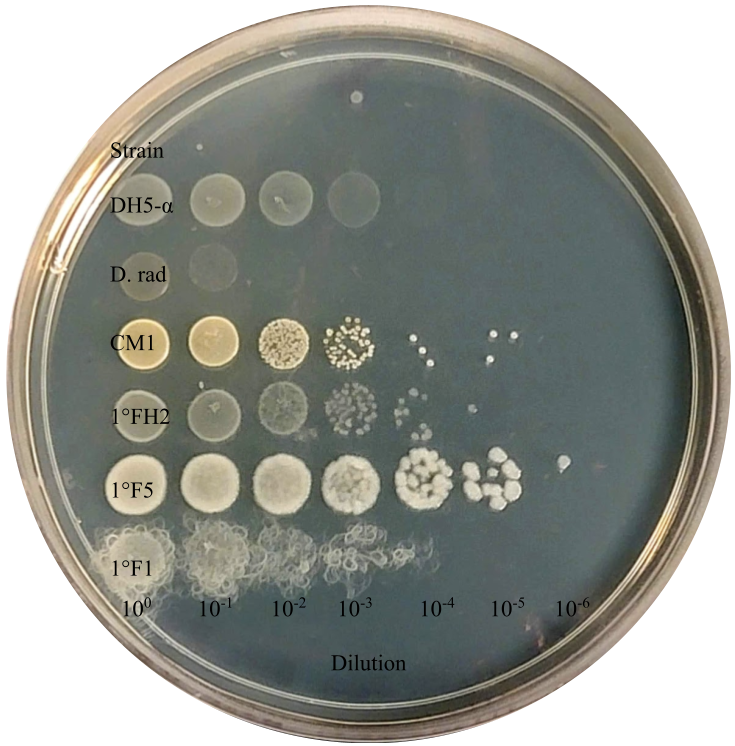
\includegraphics[width=\textwidth]{figure/0secUV.png}
\caption[0 second UV]{Growth of strains without UV interferance. Serial dilution LB plate without CFU/mL normalization, unexposed to UV light, and after overnight growth at 30$^\circ$C. Serial dilutions were made using fresh overnight cultures and LB. Each strain is labeled with their own row, and dilutions are labeld for each column.}
\label{fig:0secUV}
\end{figure}
\begin{figure}[t]
\centering
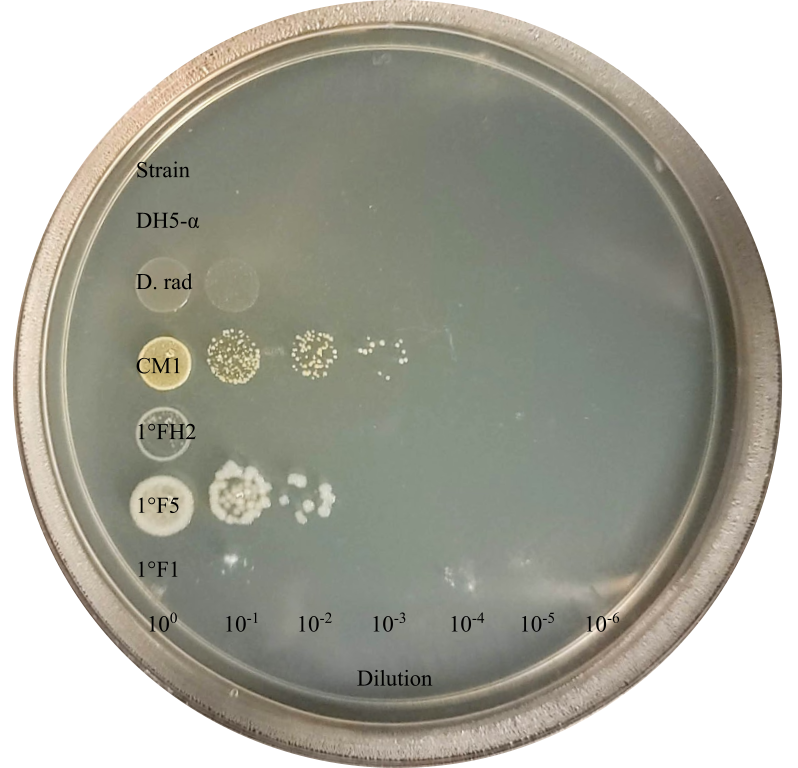
\includegraphics[width=\textwidth]{figure/60secUV.png}
\caption[60 second UV]{Growth of strains with UV interferance. Serial dilution LB plate without CFU/mL normalization, exposed to UV light for 60 seconds, and after overnight growth at 30$^\circ$C. Serial dilutions were made using fresh overnight cultures and LB. Each strain is labeled with their own row, and dilutions are labeld for each column.}
\label{fig:60secUV}
\end{figure}
\begin{figure}
\centering
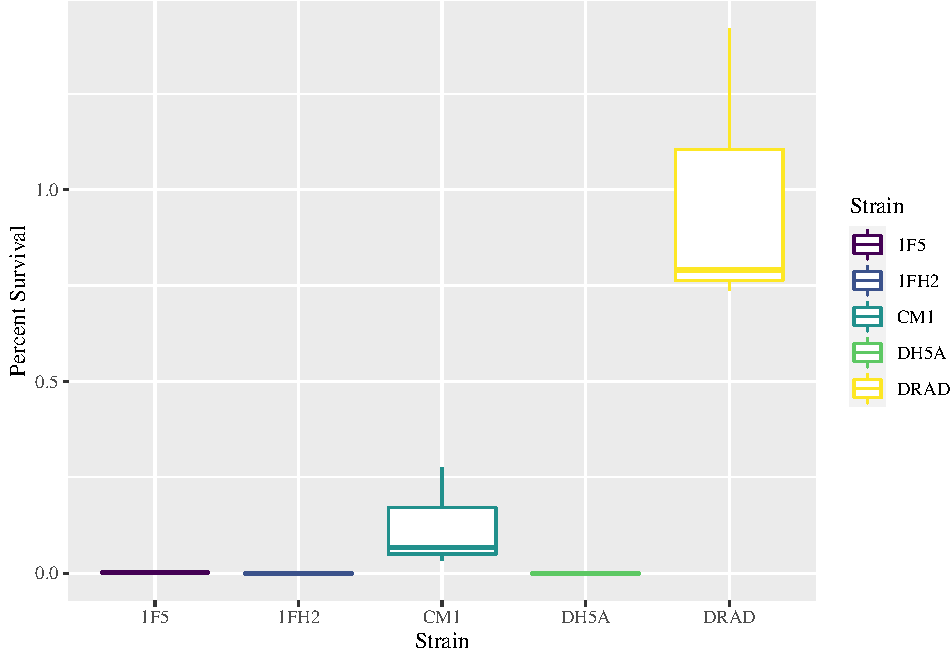
\includegraphics{thesis_files/figure-latex/sz_uv-1.pdf}
\caption{(\#fig:sz\_uv)Percent Survival of Strains in UV irradiation. For each strain, sets of three serial dilution plates were either exposed to UV for 60 seconds or not exposed at all. The CFU/mL were calculated and used to graph percent survival. Each boxplot consists of three percent survival values from each set of plates. This figure was produced using RStudio, ggplot, and Viridis.}
\end{figure}
The first several rounds of UV irradiation showed considerable differences in percent survival for the three strains 1\(^{\circ}\)F5, 1\(^{\circ}\)FH2, and CM1, and the controls D. rad and DH5-\(\alpha\) (Figure @ref\{fig:sz\_uv\}). The colony counts were taken into consideration with time exposed to calculated percent survival for each strain to compare relative radioresistance (Figures \ref(fig:0secUV) and \ref(fig:60secUV)). It was noticed, however, that there was a significant difference in CFU/mL post exposure in the same dilutions (10 colonies for 1\(^\circ\)FH2 versus 3 colonies for CM1 in the \(10^{-4}\) dilutions for example, Figure \ref(fig:0secUV)). This caused concern about confounding variables such as growth rate for different strains as well as the difference in standard CFU/mL for overnight cultures. While these initial assays proved basic radioresistance for lightly regulated conditions, they also provided a strong basis for further experimentation.

The t-tests run for this set of data compared average CFU/mL within strains between 60 seconds and 0 seconds of UV exposure. For t-tests the higher the t-value, the larger the difference that exists between the two samples. In Table \ref{tab:ttests1}, the t-test values from largest to smallest correspond to DH5-\(\alpha\), 1\(^\circ\)FH2, 1\(^\circ\)F5, CM1, then D. rad. This means that DH5-\(\alpha\) saw the largest change in CFU/mL caused by UV exposure and D. rad saw the least, as expected for the negative and positive radioresistant controls, respectively. Paired with the analysis of P-values at the significance level of \(\alpha = 0.05\) (or \(\alpha = 5.0*10^{-2}\) to compare for scientific notation), only DH5-\(\alpha\) and 1\(^\circ\)FH2 do not make the cutoff. Failing to make the cutoff for P-value significance means that strains DH5-\(\alpha\) and 1\(^\circ\)FH2 do not maintain similar means with and without UV exposure. Long story short, this data tells us that DH5-\(\alpha\) and 1\(^\circ\)FH2 are not radioresistant, whereas the others may be.
\begin{longtable}[t]{lrrrr}
\caption[T-Tests Non-normalized]{\label{tab:ttests1} Welch’s two Sample t-test of CFU/mL from serial dilutions without normalizing}\\
\toprule
Strain & Mean at 0 sec & Mean at 60 Sec & T value & P value\\
\midrule
DH5A & 4.70e+07 & 0.00e+00 & 9.54e+00 & 1.08e-02\\
DRAD & 5.67e+05 & 5.56e+05 & 6.52e-02 & 9.52e-01\\
CM1 & 1.60e+06 & 1.08e+05 & 2.00e+00 & 1.84e-01\\
1FH2 & 6.44e+05 & 3.33e+01 & 6.20e+00 & 2.51e-02\\
1F5 & 5.52e+06 & 9.33e+03 & 2.93e+00 & 9.94e-02\\
\bottomrule
\end{longtable}
\hypertarget{growth-rates}{%
\section{Growth Rates}\label{growth-rates}}

To tackle the first issue of different growth rates across strains, an overnight absorbency assay was run to calculate doubling times and ensure the show of radioresistance (or lack thereof) was not confused with slower growing characteristics of strains. The Tecan run yielded the absorbances of the strains' liquid cultures over the course of 24 hours at 30\(^\circ\)C to show the growth curves in Figure \ref{fig:tecan}.

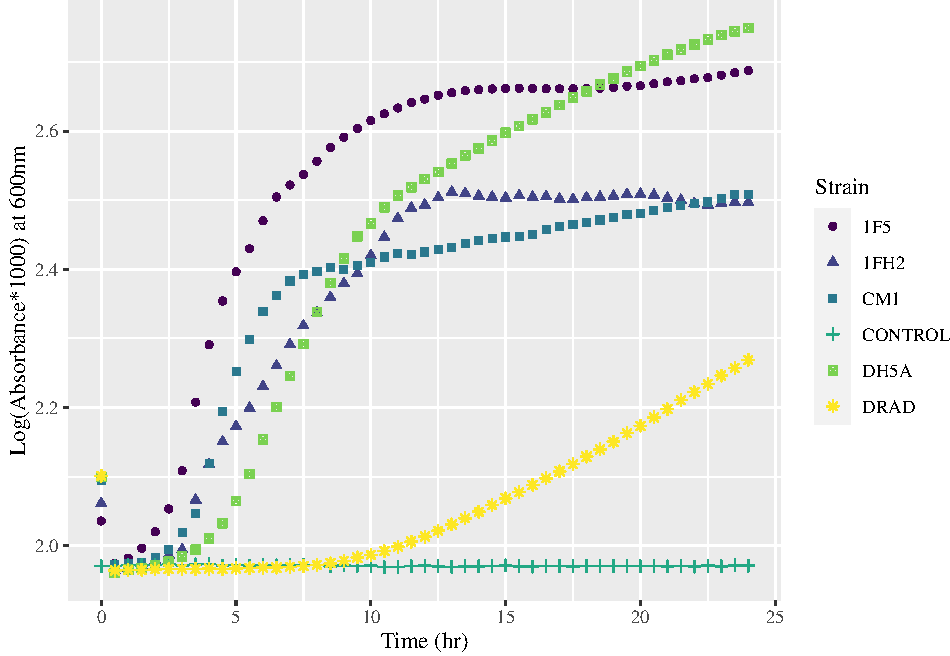
\includegraphics{thesis_files/figure-latex/tecan-1.pdf}
To calculate doubling time, the logarithmic growth portions of the curve were analyzed for the slope with highest linear fit. To ensure efficiency and accuracy, a script was written to consistently find the most linear portions of the curves (see Appendix for details/code). The selected points are show in Figure @ref(fig:tecan\_linear), and the slopes were plugged into Equation \ref{eq:doubling} to calculate the doubling times in Table @ref(tab:lm\_doubling).
\begin{verbatim}
`geom_smooth()` using formula 'y ~ x'
\end{verbatim}
\begin{figure}
\centering
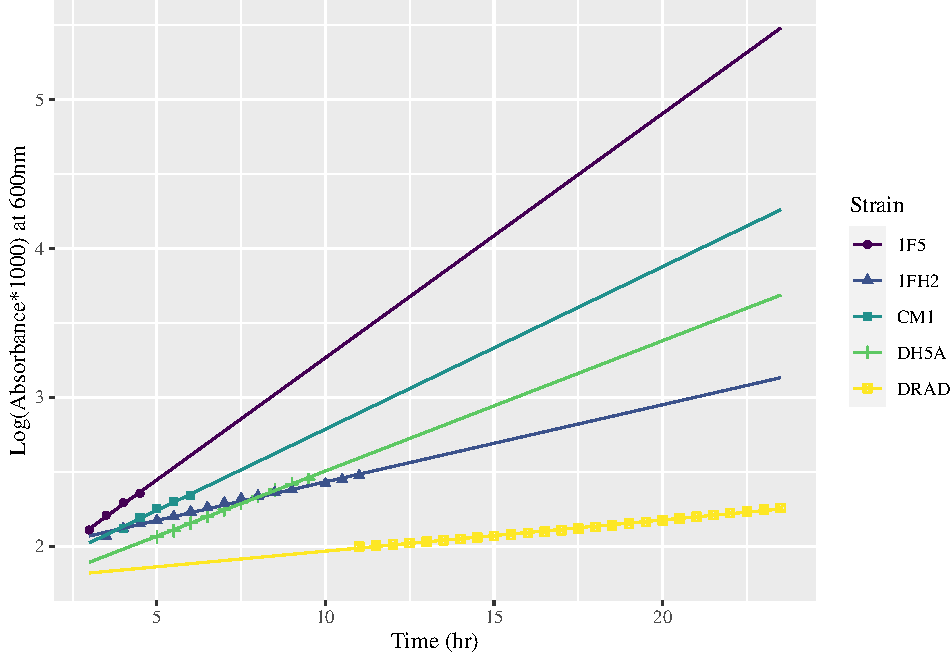
\includegraphics{thesis_files/figure-latex/tecan_linear-1.pdf}
\caption{(\#fig:tecan\_linear)Linear Portion of Growth Curves from 24 hour Tecan Run in LB. Filtered from the previous graph is the log-growth portion of the bacterial growth curves. Linear models were optimized by analyzing for the best regression values for adjacent collections of points. This figure was produced using RStudio, ggplot, and Viridis.}
\end{figure}
\textbackslash begin\{longtable\}{[}t{]}\{lrrr\}
\textbackslash caption{[}Doubling Times{]}\{(\#tab:lm\_doubling)Linear Regression Models and Calculated Doubling Times\}\textbackslash{}
\toprule
Strain \& Slope \& Doubling Time (hr) \& R Squared\textbackslash{}
\midrule
DH5A \& 0.088 \& 3.440 \& 0.997\textbackslash{}
DRAD \& 0.021 \& 14.365 \& 0.996\textbackslash{}
1F5 \& 0.115 \& 2.624 \& 0.959\textbackslash{}
1FH2 \& 0.052 \& 5.807 \& 0.990\textbackslash{}
CM1 \& 0.109 \& 2.759 \& 0.979\textbackslash{}
\bottomrule
\textbackslash end\{longtable\}

The strain with fastest growth was 1\(^{\circ}\)F5 and D. rad was the slowest growing, which could be observed on the plates, as colonies were often confluent for 1\(^{\circ}\)F5 and sparse for D. rad despite both showing indications of radioresistance. This could be due to much higher CFU/mL in overnight cultures, as they did not grow to the capacity of the liquid media. The two controls, DH5-\(\alpha\) and D. rad, also portrayed different rates, which aligned with the observation of more growth of DH5-\(\alpha\) than D. rad on unexposed plates. This confirms that the absence of DH5-\(\alpha\) in exposed plates was not due to slow growth rates, but from radiation damage. Using information from growth rates, further characterization of strains was performed in addition to secondary analysis of initial plate exposures after this information was processed.

\hypertarget{radioresistance-part-2-electric-bungaloo}{%
\section{Radioresistance Part 2: electric bungaloo}\label{radioresistance-part-2-electric-bungaloo}}

Armed with the knowledge of growth rate, fresh serial dilutions were performed to determine the CFU/mL of each overnight culture. The counts were then used to determine the starting CFU/mL for all strains at \(10^0\) dilution. This similar CFU/mL across dilutions when not irradiated allowed for direct comparison while taking into account growth rates via normalization of concentrations.
\begin{figure}[t]
\centering
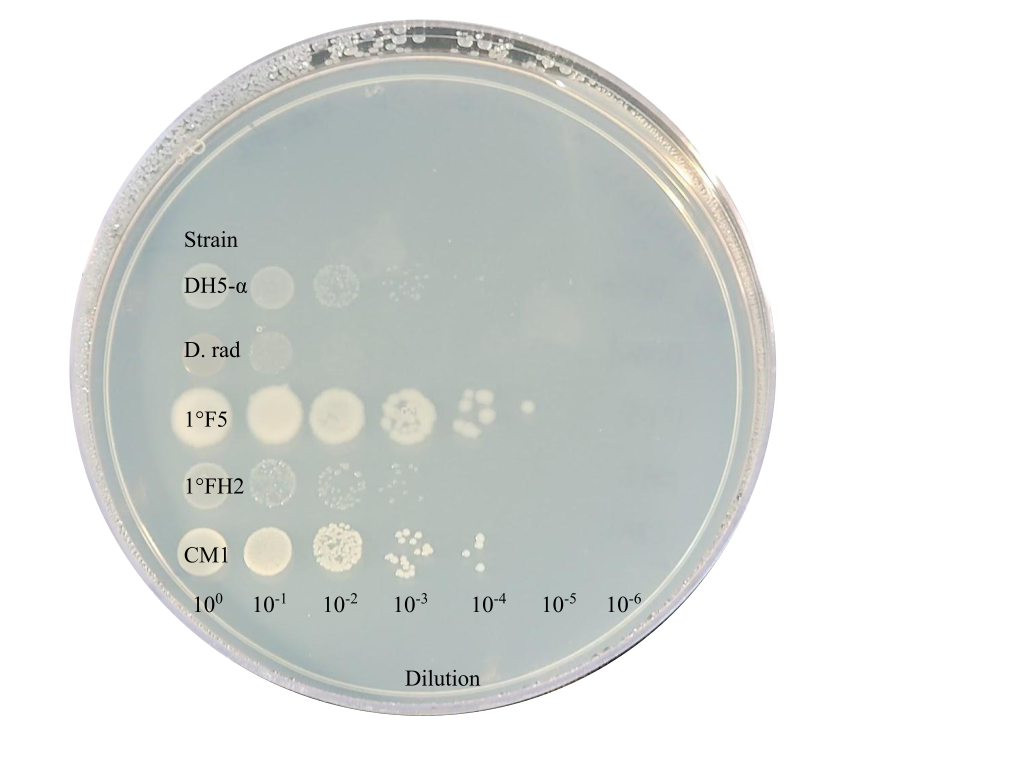
\includegraphics[width=\textwidth]{figure/n0secUV.png}
\caption[Normalized UV - 0 seconds]{}
\label{fig:n0secUV}
\end{figure}
\begin{figure}[t]
\centering
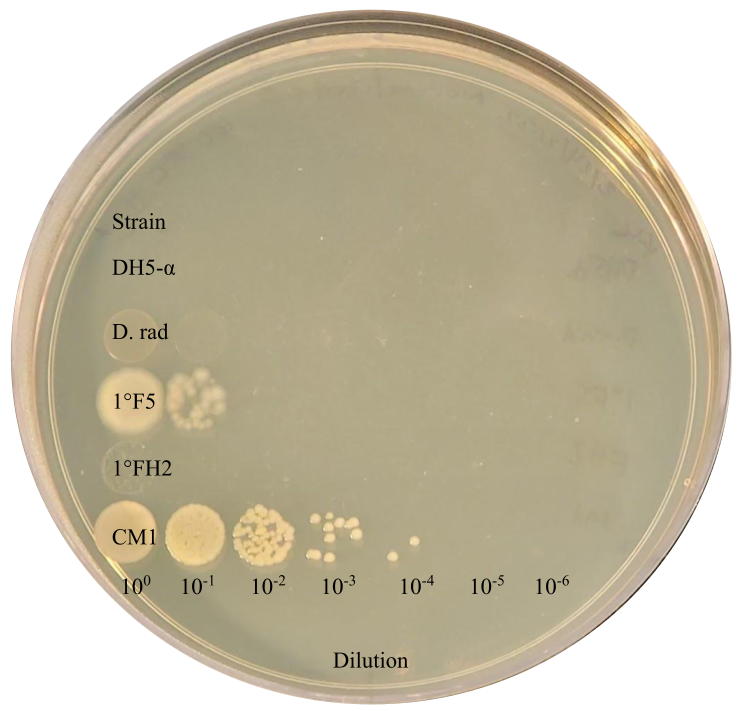
\includegraphics[width=\textwidth]{figure/n60secUV.png}
\caption[Normalized UV - 60 seconds]{}
\label{fig:n60secUV}
\end{figure}
There is a noticeable difference in growth for 1\(^\circ\)F5 after serial dilutions were normalized that can be seen when comparing Figures \ref(fig:60secUV) and \ref(fig:n60secUV). This indicates that the radioresistance observed in the first set of assays was from fast growth or high starting bacterial concentration rate rather than radioresistance. 1\(^\circ\)FH2 also had a slight change in growth density between Figures \ref(fig:60secUV) and \ref(fig:n60secUV), but that may be attributed to easier counting in dilutions now that CFU/mL was normalized. Before normalization, there would only be a semi confluent area that did not allow for accurate quantification. The normalized assay also brings to light the higher radioresistance of CM1 compared to the other isolates that was not observed to be as close to the survival rate of D. rad previously (Figure @ref(fig:n\_sz\_uv)). The controls D. rad and DH5-alpha remained consistent for both assays, as they were slightly slower growing than the other isolates and had distinct colonies that were easily countable. If anything, D. rad seemed to have an even higher percent survival (with an average closer to 150\% survival than 100\% survival in Figure @ref(fig:n\_sz\_uv)) than the non-normalized assay. Whether this detail has to do with radioresistance or radiation promoted growth is unknown.
\begin{figure}
\centering
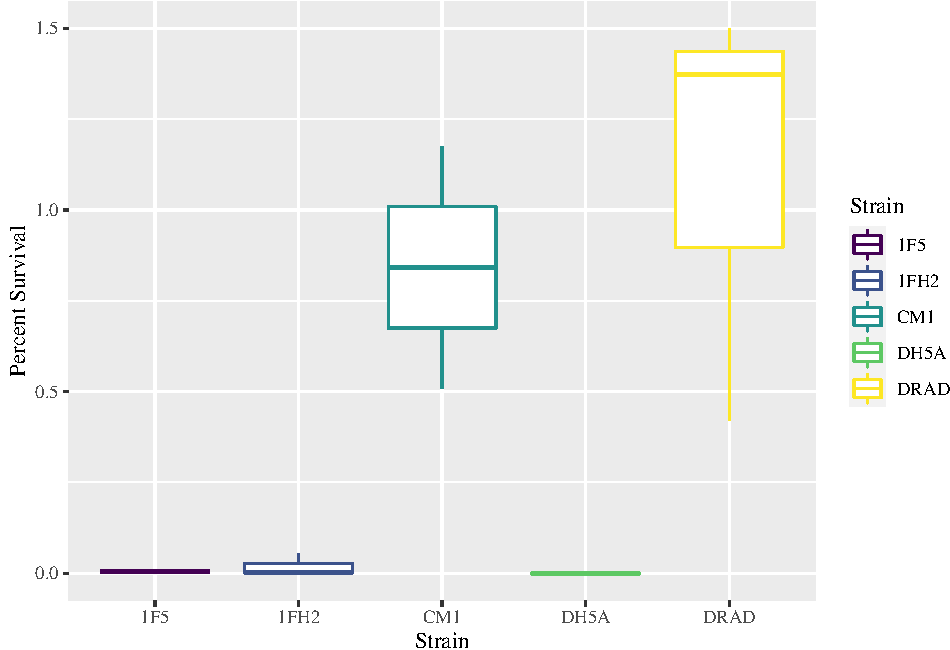
\includegraphics{thesis_files/figure-latex/n_sz_uv-1.pdf}
\caption{(\#fig:n\_sz\_uv)Percent Survival of Normalized Strains in UV irradiation. For these serial dilutions, the starting concentration for all strains was \(2.2*10^5\) CFU/mL to ensure that concentration of starting culture would not be a confounding variable in calculating and comparing percent survival. Again, for each strain, sets of three serial dilution plates were either exposed to UV for 60 seconds or not exposed at all. The CFU/mL were calculated and used to graph percent survival. Each boxplot consists of three percent survival values from each set of plates. This figure was produced using RStudio, ggplot, and Viridis.}
\end{figure}
Welch's two sample t-test was again run for the average CFU/mL between UV exposure states for each strain. Things of note this time in Table \ref{tab:ttests2} are that both D. rad and CM1 have very low t-values and very high P-values compared to the other strains. In addition to that, DH5-\(\alpha\) has a high t-value, but not a statistically significant P-value. This means that while there is a large change in CFU/mL cause by UV exposure, but something isn't quite right.
\begin{longtable}[t]{lrrrr}
\caption[T-Tests Normalized]{\label{tab:ttests2}Welch’s two Sample t-test of CFU/mL from serial dilutions with normalizing}\\
\toprule
Strain & Mean at 0 sec & Mean at 60 Sec & T value & P value\\
\midrule
DH5A & 2.98e+05 & 0.00e+00 & 2.51e+00 & 1.3e-01\\
DRAD & 4.23e+05 & 3.67e+05 & 3.68e-01 & 7.4e-01\\
CM1 & 3.33e+05 & 2.89e+05 & 3.16e-01 & 8.0e-01\\
1FH2 & 3.95e+05 & 6.67e+02 & 6.20e+00 & 3.0e-02\\
1F5 & 8.17e+05 & 4.30e+03 & 4.86e+01 & 0.0e+00\\
\bottomrule
\end{longtable}
This P-value was unexpected because it indicates that DH5-\(\alpha\) colony counts could not lead to conclusive evidence to either reject nor accept the null-hypothesis that there is no change in mean CFU/mL with and without UV exposure. Looking back into the raw data, an outlier is present in Table @ref(tab:dh5a\_noUV) Strain 2, for the \(10^-5\) dilution. While the other values generally are comparable between each set, the single colony is \(10^-5\) could either have been a miscount, an experimental error, or just a resilient colony. Either way, without more repetitions, the P-value in Table \ref{tab:ttests2} for DH5-\(\alpha\) should be taken with a grain of salt.

\textbackslash begin\{longtable\}{[}t{]}\{rrrr\}
\textbackslash caption{[}DH5A without UV{]}\{(\#tab:dh5a\_noUV)Colony Counts for DH5A Without UV Exposure\}\textbackslash{}
\toprule
Set \& Colonies \& Dilution \& CFU/mL\textbackslash{}
\midrule
1 \& 21 \& -3 \& 210000\textbackslash{}
1 \& 1 \& -4 \& 100000\textbackslash{}
2 \& 20 \& -3 \& 200000\textbackslash{}
2 \& 4 \& -4 \& 400000\textbackslash{}
2 \& 1 \& -5 \& 1000000\textbackslash{}
\addlinespace
3 \& 21 \& -3 \& 210000\textbackslash{}
3 \& 2 \& -4 \& 200000\textbackslash{}
\bottomrule
\textbackslash end\{longtable\}
Table \ref{tab:ttests2} does aid in observing that 1\(^\circ\)F5 no longer seems as radioresistant as it did in Table \ref{tab:ttests1}, as it now had the largest t-value and smallest p-value of the strains isolated for this study. Again, this indcates that the observed radioresistance in the first set of UV serial dilutions (Figure \ref(fig:60secUV)) could have been caused by high bacterial density in the starting \(10^0\) dilution, allowing more growth after exposure to UV. At the significance level of \(\alpha = 0.05\), we can conclude that only D. rad and CM1 are unaffected by UV exposure, and though the P-value of DH5-\(\alpha\) is above the significance level, the corresponding t-value indicates a large difference between the number of colonies found without UV exposure and the number of colonies (or lack thereof) with UV exposure.

The normalized serial dilutions proved invaluable in accurately assessing the radioresistance of bacterial strains by taking growth conditions and growth rates into account. This final UV assay confirmed strong radioresistance in CM1 compared to the other isolated RRR strains. The next step is to identify the species of CM1 and any DNA-repair mechanisms that it has developed while living in the pool of a nuclear reactor.

\hypertarget{identification}{%
\section{Identification}\label{identification}}

\hypertarget{gram-stains}{%
\subsection{Gram Stains}\label{gram-stains}}

Gram stains performed on isolates revealed they were all rod-shaped, gram positive bacteria. It also allowed for basic measurements of bacteria using stage micrometers, as shown in Figure \ref(fig:GramStain). This information aided in narrowing down potential strains with 16S sequencing. The strains in this study, CM1, 1\(^\circ\)F5, and 1\(^\circ\)FH2, are all Gram-negative bacteria. This means that they all have two layers of membranes and are less susceptible antibiotics and lysing agents. For this study in particular, this made DNA isolation of CM1 for genome analysis more difficult, with lower DNA concentration yield.
\begin{figure}[t]
\centering
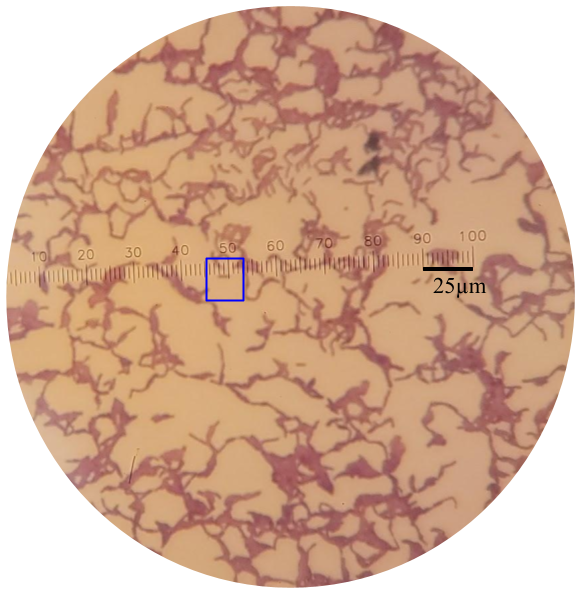
\includegraphics[width=\textwidth]{figure/GramStain.png}
\caption[CM1 Gram Stain]{Gram stain of strain CM1 at 400x magnification. A line equal to the length of 10 units demarcated on the lens is indicated on the image in black font to be 25 $\mu$m. A single bacterium is boxed close and lined up with the tick-marks to show that the size is approximately 5 $\mu$m. The purple color of the stained cells indicate that CM1 is Gram-negative and features both an outer membrane and a cytoplamic membrane, rather than a cytoplasmic membrane and a thick peptidoglycan layer.}
\label{fig:GramStain}
\end{figure}
\hypertarget{s-pcr}{%
\subsection{16S PCR}\label{s-pcr}}

For genus level identification of isolates, 16S PCR and sequencing was performed. After receiving the 16S sequences from ACGT, Inc., the NCBI blasts showed many matches to various \emph{Baccili} strains. Using the percent identities and E scores indicating levels of matching in addition to visual qualification of bacteria through colony characteristics and size of bacterium, a very general idea of species was hypothesized, as shown in Table \ref{tab:blasts}. In addition to 16S sequencing, CM1 will also undergo whole genome sequencing, as it is the most radioresistant. These results aided in preparing information such as a reference genome for WGS analysis.
\begin{verbatim}
Warning in read.table(file = file, header = header, sep = sep, quote
= quote, : incomplete final line found by readTableHeader on '/Users/
kaitlynli/Documents/Reed Year 4/Thesis/RRR_Bacteria/data/blasts.csv'
\end{verbatim}
\begin{longtable}[t]{lll}
\caption[Hypothesized Identification]{\label{tab:blasts}Hypothesized identification of isolates in this study based off 16S sequencing}\\
\toprule
Isolate & Suggested Genus & Suggested Species\\
\midrule
CM1 & Bacillus, Priestia & B. megaterium, P. megaterium\\
1FH2 & Lysinibacillus & L. xylanilyticus, L. subtilis\\
1F5 & Bacillus & B. cereus, B. thuringiensis\\
1F1 & Bacillus & B. pseudomycoides, B. mycoides\\
\bottomrule
\end{longtable}
\hypertarget{whole-genome-analysis-of-cm1}{%
\subsection{Whole Genome Analysis of CM1}\label{whole-genome-analysis-of-cm1}}

As whole genome data was not received until near the end of this study, the following results are but surface-level analysis of the sequenced genome.

\hypertarget{conclusion}{%
\chapter{Conclusion}\label{conclusion}}

In this study, I explored organisms living in extreme environments, such as the water systems of nuclear reactors, and the possibility of observing their genome for unique methods of resistance to ionizing radiation, whether it be through mechanisms of protection against radiation-induced oxidative damage to proteins, or repair of such damage. Strain CM1 of Priestia Megaterium is a robust bacterium isolated from surfaces surrounding the core of the Reed Research Reactor. Of the 10 strains isolated from various areas of the RRR water system, only CM1 was radioresistant enough to portray the same level of growth as Deinococcus radiodurans when calculating survivability and growth rates. The radioresistance of CM1 was tested by UV light against controls DH5-a and Deinococcus radiodurans using serial dilution and growth assays to assess survivability and growth rates affected by exposure to UV light. Identification on a genus based level was performed via 16S analysis and sequencing by ACGT (ACGT, Inc., Wheeling, IL), and its genome was sequenced by Novogene (Novogene Corporation Inc., Sacramento, CA).
The results of my experiments have laid groundwork for future studies with this strain of radioresistant bacteria. Not only have we found more information on species on mutations from the reference genome, but also the specific genes that have changed. \emph{From the BLANK gene mutations observed, function of the produced proteins can be experimentally tested under radioactive stress. In addition to that, more samples of this bacteria can be isolated from period samples of RRR water to observe mutations over time near the core of a nuclear reactor. {[}{[}MORE ABOUT GENOME ANALYSIS RESULTS{]}{]} While the mechanisms of survival have not been elucidated in this study, sequencing the genome allows for future studies such as protein knock-out assays that can help figure out which proteins or mechanisms are responsible for the survivability of this bacteria. This work has already begun through the study of the ATP-dependent RecD-like DNA helicase of CM1 (N. Xu and H. Monyatovsky, unpublished data).}
Search for more efficient methods of radioactive waste cleanup has been in progress since the 1900s with the nuclear industry boom (17). Both bacteria and fungi have been studied for bioabsorption and remediation of radionuclides through accumulation of contaminants in life and death. Biopolymers and biosorption using biomass have great potential for not just nuclear waste treatment, but waste treatment in general. In more recent publications than a paper from 1989, an increase in uranium contamination as chemical toxicity and radioactivity is slowly creeping its way from power plants and uranium mills to the top of the food chain in the form of oxides, precipitates, complexes, and natural minerals. Researchers have observed uptake of uranium oxide through biosorption and biomineralization by Bacillus subtilis ATCC-6633 (18) and the environmental conditions for bioreduction by numerous other microorganisms (19). Radioresistant bacteria are constantly being discovered, including at least 100 from the Taklimakan Desert in a paper published March 2022 (20).
With new textbooks, research, and articles being published on bioremediation of radioactive waste, there's a long way to go for efficient usage of these materials. With the work done in this study, I hope that one day it can contribute to creating consortiums of bacteria used to take care of mixed wastes, to combine with the research of plastic degradation, chemical wastes, and biological waste. Looking for bacteria in harsh environments such as nuclear reactor facilities or the hottest deserts in the world can help with the extreme conditions we've created for Earth. Just as scientists have searched for bacteriophages in hospital sewage as cures for bacterial infections (21), just as the Toxic Jungle cleanses the air for the Valley of the Wind (22), working with tools given by the environment can be key to solving many of the world's waste crises.

\hypertarget{conclusion-1}{%
\chapter*{Conclusion}\label{conclusion-1}}
\addcontentsline{toc}{chapter}{Conclusion}

If we don't want Conclusion to have a chapter number next to it, we can add the \texttt{\{-\}} attribute.

\textbf{More info}

And here's some other random info: the first paragraph after a chapter title or section head \emph{shouldn't be} indented, because indents are to tell the reader that you're starting a new paragraph. Since that's obvious after a chapter or section title, proper typesetting doesn't add an indent there.

\appendix

\hypertarget{the-first-appendix}{%
\chapter{The First Appendix}\label{the-first-appendix}}

This first appendix includes all of the R chunks of code that were hidden throughout the document (using the \texttt{include\ =\ FALSE} chunk tag) to help with readibility and/or setup.

\textbf{In the main Rmd file}
\begin{Shaded}
\begin{Highlighting}[]
\NormalTok{knitr}\OperatorTok{::}\NormalTok{opts_chunk}\OperatorTok{$}\KeywordTok{set}\NormalTok{(}\DataTypeTok{echo =} \OtherTok{FALSE}\NormalTok{)}
\CommentTok{# This chunk ensures that the thesisdown package is}
\CommentTok{# installed and loaded. This thesisdown package includes}
\CommentTok{# the template files for the thesis.}
\ControlFlowTok{if}\NormalTok{ (}\OperatorTok{!}\KeywordTok{require}\NormalTok{(remotes)) \{}
  \ControlFlowTok{if}\NormalTok{ (params}\OperatorTok{$}\StringTok{`}\DataTypeTok{Install needed packages for \{thesisdown\}}\StringTok{`}\NormalTok{) \{}
    \KeywordTok{install.packages}\NormalTok{(}\StringTok{"remotes"}\NormalTok{, }\DataTypeTok{repos =} \StringTok{"https://cran.rstudio.com"}\NormalTok{)}
\NormalTok{  \} }\ControlFlowTok{else}\NormalTok{ \{}
    \KeywordTok{stop}\NormalTok{(}
      \KeywordTok{paste}\NormalTok{(}\StringTok{'You need to run install.packages("remotes")",}
\StringTok{            "first in the Console.'}\NormalTok{)}
\NormalTok{    )}
\NormalTok{  \}}
\NormalTok{\}}
\ControlFlowTok{if}\NormalTok{ (}\OperatorTok{!}\KeywordTok{require}\NormalTok{(dplyr)) \{}
  \ControlFlowTok{if}\NormalTok{ (params}\OperatorTok{$}\StringTok{`}\DataTypeTok{Install needed packages for \{thesisdown\}}\StringTok{`}\NormalTok{) \{}
    \KeywordTok{install.packages}\NormalTok{(}\StringTok{"dplyr"}\NormalTok{, }\DataTypeTok{repos =} \StringTok{"https://cran.rstudio.com"}\NormalTok{)}
\NormalTok{  \} }\ControlFlowTok{else}\NormalTok{ \{}
    \KeywordTok{stop}\NormalTok{(}
      \KeywordTok{paste}\NormalTok{(}
        \StringTok{'You need to run install.packages("dplyr")'}\NormalTok{,}
        \StringTok{"first in the Console."}
\NormalTok{      )}
\NormalTok{    )}
\NormalTok{  \}}
\NormalTok{\}}
\ControlFlowTok{if}\NormalTok{ (}\OperatorTok{!}\KeywordTok{require}\NormalTok{(ggplot2)) \{}
  \ControlFlowTok{if}\NormalTok{ (params}\OperatorTok{$}\StringTok{`}\DataTypeTok{Install needed packages for \{thesisdown\}}\StringTok{`}\NormalTok{) \{}
    \KeywordTok{install.packages}\NormalTok{(}\StringTok{"ggplot2"}\NormalTok{, }\DataTypeTok{repos =} \StringTok{"https://cran.rstudio.com"}\NormalTok{)}
\NormalTok{  \} }\ControlFlowTok{else}\NormalTok{ \{}
    \KeywordTok{stop}\NormalTok{(}
      \KeywordTok{paste}\NormalTok{(}
        \StringTok{'You need to run install.packages("ggplot2")'}\NormalTok{,}
        \StringTok{"first in the Console."}
\NormalTok{      )}
\NormalTok{    )}
\NormalTok{  \}}
\NormalTok{\}}
\ControlFlowTok{if}\NormalTok{ (}\OperatorTok{!}\KeywordTok{require}\NormalTok{(bookdown)) \{}
  \ControlFlowTok{if}\NormalTok{ (params}\OperatorTok{$}\StringTok{`}\DataTypeTok{Install needed packages for \{thesisdown\}}\StringTok{`}\NormalTok{) \{}
    \KeywordTok{install.packages}\NormalTok{(}\StringTok{"bookdown"}\NormalTok{, }\DataTypeTok{repos =} \StringTok{"https://cran.rstudio.com"}\NormalTok{)}
\NormalTok{  \} }\ControlFlowTok{else}\NormalTok{ \{}
    \KeywordTok{stop}\NormalTok{(}
      \KeywordTok{paste}\NormalTok{(}
        \StringTok{'You need to run install.packages("bookdown")'}\NormalTok{,}
        \StringTok{"first in the Console."}
\NormalTok{      )}
\NormalTok{    )}
\NormalTok{  \}}
\NormalTok{\}}
\ControlFlowTok{if}\NormalTok{ (}\OperatorTok{!}\KeywordTok{require}\NormalTok{(thesisdown)) \{}
  \ControlFlowTok{if}\NormalTok{ (params}\OperatorTok{$}\StringTok{`}\DataTypeTok{Install needed packages for \{thesisdown\}}\StringTok{`}\NormalTok{) \{}
\NormalTok{    remotes}\OperatorTok{::}\KeywordTok{install_github}\NormalTok{(}\StringTok{"ismayc/thesisdown"}\NormalTok{)}
\NormalTok{  \} }\ControlFlowTok{else}\NormalTok{ \{}
    \KeywordTok{stop}\NormalTok{(}
      \KeywordTok{paste}\NormalTok{(}
        \StringTok{"You need to run"}\NormalTok{,}
        \StringTok{'remotes::install_github("ismayc/thesisdown")'}\NormalTok{,}
        \StringTok{"first in the Console."}
\NormalTok{      )}
\NormalTok{    )}
\NormalTok{  \}}
\NormalTok{\}}

\KeywordTok{library}\NormalTok{(thesisdown)}
\KeywordTok{library}\NormalTok{(dplyr)}
\KeywordTok{library}\NormalTok{(ggplot2)}
\KeywordTok{library}\NormalTok{(graphics)}
\KeywordTok{library}\NormalTok{(knitr)}
\KeywordTok{library}\NormalTok{(viridis)}
\CommentTok{# Set how wide the R output will go}
\KeywordTok{options}\NormalTok{(}\DataTypeTok{width =} \DecValTok{70}\NormalTok{)}
\end{Highlighting}
\end{Shaded}
\textbf{In Chapter \ref{ref-labels}:}

\hypertarget{the-second-appendix-for-fun}{%
\chapter{The Second Appendix, for Fun}\label{the-second-appendix-for-fun}}

\backmatter

\hypertarget{references}{%
\chapter*{References}\label{references}}
\addcontentsline{toc}{chapter}{References}

\markboth{References}{References}

\noindent

\setlength{\parindent}{-0.20in}

\hypertarget{refs}{}
\leavevmode\hypertarget{ref-noauthor_many_nodate}{}%
1. The Many Uses of Nuclear Technology - World Nuclear Association.

\leavevmode\hypertarget{ref-cember_introduction_1996}{}%
2. Cember H. 1996. Introduction to Health Physics3rd edition. McGraw-Hill Medical, New York.

\leavevmode\hypertarget{ref-iqbal_thyroid_2022}{}%
3. Iqbal A, Rehman A. 2022. Thyroid Uptake and Scan. \emph{In} StatPearls. StatPearls Publishing, Treasure Island (FL).

\leavevmode\hypertarget{ref-zhdanova_ionizing_2004}{}%
4. Zhdanova NN, Tugay T, Dighton J, Zheltonozhsky V, McDermott P. 2004. Ionizing radiation attracts soil fungi. Mycological Research 108:1089--1096.

\leavevmode\hypertarget{ref-binks_radioresistant_1996}{}%
5. Binks PR. 1996. Radioresistant bacteria: Have they got industrial uses? Journal of Chemical Technology \& Biotechnology 67:319--322.

\leavevmode\hypertarget{ref-cologgi_extracellular_2011}{}%
6. Cologgi DL, Lampa-Pastirk S, Speers AM, Kelly SD, Reguera G. 2011. Extracellular reduction of uranium via Geobacter conductive pili as a protective cellular mechanism. Proceedings of the National Academy of Sciences 108:15248--15252.

\leavevmode\hypertarget{ref-koribanics_spatial_2015}{}%
7. Koribanics NM, Tuorto SJ, Lopez-Chiaffarelli N, McGuinness LR, Häggblom MM, Williams KH, Long PE, Kerkhof LJ. 2015. Spatial Distribution of an Uranium-Respiring Betaproteobacterium at the Rifle, CO Field Research Site. PLOS ONE 10:e0123378.

\leavevmode\hypertarget{ref-krisko_biology_2013}{}%
8. Krisko A, Radman M. 2013. Biology of Extreme Radiation Resistance: The Way of Deinococcus radiodurans. Cold Spring Harbor Perspectives in Biology 5.

\leavevmode\hypertarget{ref-witkin_inherited_1946}{}%
9. Witkin EM. 1946. Inherited Differences in Sensitivity to Radiation in Escherichia coli. Proceedings of the National Academy of Sciences of the United States of America 32:59--68.

\leavevmode\hypertarget{ref-dadachova_ionizing_2007}{}%
10. Dadachova E, Bryan RA, Huang X, Moadel T, Schweitzer AD, Aisen P, Nosanchuk JD, Casadevall A. 2007. Ionizing Radiation Changes the Electronic Properties of Melanin and Enhances the Growth of Melanized Fungi. PLOS ONE 2:e457.

\leavevmode\hypertarget{ref-bruckbauer_experimental_2021}{}%
11. Bruckbauer ST, Cox MM. 2021. Experimental evolution of extremophile resistance to ionizing radiation. Trends in Genetics 37:830--845.

\leavevmode\hypertarget{ref-yang_microbial_2021}{}%
12. Yang X, Li S, Song G, Xu X, Hu D. 2021. Microbial diversity formed and maintained through substrate feedback regulation and delayed responses induced by Low-Dose Ionizing Radiation. Acta Astronautica 188:239--251.

\leavevmode\hypertarget{ref-shahbazi-gahrouei_review_2013}{}%
13. Shahbazi-Gahrouei D, Gholami M, Setayandeh S. 2013. A review on natural background radiation. Advanced Biomedical Research 2:65.

\leavevmode\hypertarget{ref-chicote_isolation_2005}{}%
14. Chicote E, García AM, Moreno DA, Sarró MI, Lorenzo PI, Montero F. 2005. Isolation and identification of bacteria from spent nuclear fuel pools. Journal of Industrial Microbiology and Biotechnology 32:155--162.

\leavevmode\hypertarget{ref-kroes_bacterial_1999}{}%
15. Kroes I, Lepp PW, Relman DA. 1999. Bacterial diversity within the human subgingival crevice. Proceedings of the National Academy of Sciences 96:14547--14552.

\leavevmode\hypertarget{ref-noauthor_priestia_nodate}{}%
16. Priestia megaterium (ID 945) - Genome - NCBI.

\leavevmode\hypertarget{ref-ashley_review_1989}{}%
17. Ashley NV, Roach DJW. 1989. Review of biotechnology applications to nuclear waste treatment. Journal of Chemical Technology \& Biotechnology 49:381--394.

\leavevmode\hypertarget{ref-song_nonreductive_2019}{}%
18. Song J, Han B, Song H, Yang J, Zhang L, Ning P, Lin Z. 2019. Nonreductive biomineralization of uranium by Bacillus subtilis ATCC--6633 under aerobic conditions. Journal of Environmental Radioactivity 208-209:106027.

\leavevmode\hypertarget{ref-wufuer_uranium_2017}{}%
19. Wufuer R, Wei Y, Lin Q, Wang H, Song W, Liu W, Zhang D, Pan X, Gadd GM. 2017. Uranium Bioreduction and Biomineralization, pp. 137--168. \emph{In} Advances in Applied Microbiology. Elsevier.

\leavevmode\hypertarget{ref-liu_high_2022}{}%
20. Liu Y, Chen T, Li J, Wu M, Liu G, Zhang W, Zhang B, Zhang S, Zhang G. 2022. High Proportions of Radiation-Resistant Strains in Culturable Bacteria from the Taklimakan Desert. Biology 11:501.

\leavevmode\hypertarget{ref-lin_phage_2017}{}%
21. Lin DM, Koskella B, Lin HC. 2017. Phage therapy: An alternative to antibiotics in the age of multi-drug resistance. World Journal of Gastrointestinal Pharmacology and Therapeutics 8:162--173.

\leavevmode\hypertarget{ref-miyazaki_nausicaa_2004}{}%
22. Miyazaki H, Thurman U, Stewart P, Lohman A, Olmos EJ. 2004. Nausicaä of the valley of the wind. Walt Disney Home Entertainment ; ~Distributed by Buena Vista Home Entertainment.


% Index?

\end{document}
